\section{N2: reconstructing explicit knowledge from the open web}
\label{sec:n2}

N2 built and stress-tested the reconstruction pipeline, \repo{reconstruct/}, that turns a
\code{(domain, task)} pair into an N1 \code{Ledger} of claim records with verified provenance. This
section reports what running it live and against adversarial harnesses showed, including the
negative and inconclusive results. \evobs{} N2's registered research verdict is
\textbf{INCONCLUSIVE}: E-PLANT's Continue branch closed on the validity floor (the ungated model adopted
$a_U = 5$ of 24 planted falsehoods, below the required 8), and the gated arms of E-PLANT and E-ABST were never scored. Separately, the engineering milestone is
complete.\footnote{\repo{research/n2/closeout.md}.}

\Cref{sec:architecture} describes the pipeline stage by stage. Two facts about it matter for
reading the results. First, every evidence item carries an exact span re-sliced from the fetched
snapshot. Extractions whose quote cannot be located stay in the ledger, labeled
\code{synthetic_extrapolation}, and can never act as a criterion. Second, the cross-verify stage and
the current decoy stage are implemented and tested offline but have never run live. The v1 runs used
the older pairwise contradiction stage, and the one post-fix run (GDPR v2) logged no cross-verify or
decoy call.\footnote{\repo{reconstruct/runs/20260928T145943Z-bc1cc9a30a02/sidecar.json}:
\code{cross_checks} and \code{decoys} are empty.} N2 ran three experiments
(\cref{tab:n2-experiments}).

\begin{table}[tbp]
  \centering
  \small
  \caption{N2's three experiments. Only E-PLANT and E-ABST are pre-registered, gated experiments;
  E-LIVE is a sanity check with no gold and no threshold.}
  \label{tab:n2-experiments}
  \begin{tabularx}{\linewidth}{@{}lXX@{}}
    \toprule
    Experiment & Question & Criterion \\
    \midrule
    E-LIVE & Does the pipeline run on the live web without fabricating, mislabeling, or falling
      over? & Inspection of runs; no gold, no threshold \\
    E-PLANT & Does gating reduce adoption of a planted false value alongside real pages? & Exact
      one-sided McNemar test, gated vs.\ ungated, with a validity floor $a_U \geq \lceil n/3 \rceil$ \\
    E-ABST & On real but private questions, does the pipeline give fewer false answers than the
      raw model? & $\mathrm{FAR}_{\text{raw}} - \mathrm{FAR}_{\text{pipe}} \geq 0.20$, with
      $n_{\text{included}} \geq 20$ \\
    \bottomrule
  \end{tabularx}
\end{table}

\subsection{E-LIVE: two domains, three run versions}

\evobs{} E-LIVE ran the pipeline on two live domains with the same model configuration:
industrial PLC intermittent-fault diagnosis (technical, procedural) and GDPR data protection impact
assessments, DPIA (legal, normative). Three versions ran: v1 (pre-fix), v2 (post-fix; the PLC run
crashed), and v3 (blocked before any billed call). \Cref{tab:n2-elive} gives the per-run
numbers.\footnote{\repo{research/n2/e_live_report.md}, \S3 and \S5; recomputed from
\repo{reconstruct/runs/}\code{<run>/sidecar.json} and \code{ledger.json}.}

\begin{table}[tbp]
  \centering
  \small
  \caption{E-LIVE per-run counts. \enquote{Located} is the sidecar's \code{n_located}, one
  definition for all runs; the ledgers hold 337, 206 and 366 evidence items (GDPR v1 and v2 hold 206 and 366
  against an \code{n_located} of 204 and 351). \enquote{Unknown claims} is
  the ledger's \code{unknown}-label count, one per (area, probe) slot that was searched, fetched and
  fully verified with nothing found; it is a different quantity from N3's \code{RG-UNK} category
  (\cref{tab:n3-results}). GDPR v2 is defect-compromised: 140 of its 366 evidence items kept a
  \code{pending} verdict after silent verifier failures, so it is not N3-admissible. PLC v2 crashed on
  a PDF encoding defect (0 claims, not shown).}
  \label{tab:n2-elive}
  \begin{tabularx}{\linewidth}{@{}lrrrrrr@{}}
    \toprule
    Run & Sources & Extracted & Located & Verified (supports) & Unknown claims & Cost \\
    \midrule
    PLC v1 & 35 & 370 & 337 & 321 & 5 & \$0.679 \\
    GDPR v1 & 20 & 259 & 204 & 195 & 14 & \$0.500 \\
    GDPR v2 & 25 & 523 & 351 & 207 & 15 & \$1.002 \\
    \bottomrule
  \end{tabularx}
\end{table}

GDPR v1's 14 of 35 (area $\times$ probe) UNKNOWN slots concentrate in \code{failure_mode} (5 of 5
areas): regulator and statute text states obligations, not how a DPIA goes wrong in practice.
\evint{} This is consistent with the kind of gap the gap map is built to flag, but it is not
validated against any ground truth.

\textbf{Exact spans.} \evobs{} The full check \code{reconstruct.verify_run} re-slices all 909
evidence items of the three completed runs exactly from their local snapshots (337 + 206 + 366). A
closeout sample by one AI inspector re-sliced 71 of 71.\footnote{\repo{research/n2/e_live_claim_inspection.md};
\repo{research/n2/e_live_report.md} \S6.2. The inspector was an AI agent, not a human. The snapshots
are git-ignored, so \code{verify_run} cannot be repeated from a fresh clone.} The claims are a
different matter. Of 1,169 claims in the three ledgers, 418 are labeled
\code{synthetic_extrapolation} (49, 64 and 305) and 34 \code{unknown}, so 452 have no supporting
span.\footnote{Labels computed with \code{ClaimRecord.label} over the three \code{ledger.json}
files.} Model-written and memorized content can therefore enter the ledger, but only under a label
that no lens and no gate reads.

\textbf{Cross-family verification.} \evobs{} A supporting verdict comes from a model of a different
family than the extractor (\code{openai/gpt-5.4-mini} vs.\ \code{anthropic/claude-haiku-4.5}), and a
same-family verdict cannot yield a criterion label. On sampled natural claims the verifier's main
error is scope drift, not fabrication: 30\% error on PLC v1 in the closeout inspection (Wilson 95\%
CI 15--52\%, $n=20$; the earlier v1 review estimated about 20\% drift), and 12\% on the current
verifier's GDPR v2 sample (Wilson 4--30\%, $n=25$, in-sample against prompts that quote these review
examples). Every GDPR drift case has one shape: a national list item is generalized to \enquote{a
DPIA is required} with the jurisdiction dropped.

\textbf{Decoy false accepts.} \evobs{} The v1 runs also tested the verifier with decoys: 20
supported claims per run, each mutated by negation, a changed number or a changed scope, and checked
again against the original span. The verifier accepted 7 of 20 decoys on PLC v1 (35\%, Wilson 95\% CI
18--57\%) and 3 of 20 on GDPR v1 (15\%, 5--36\%).\footnote{\repo{reconstruct/runs/20260928T133336Z-59ec876b3d7e/sidecar.json}
and \repo{reconstruct/runs/20260928T135354Z-eb840a85b7d1/sidecar.json}, key \code{decoys};
\repo{research/n2/e_live_review_notes.md} \S10.} On PLC, all 5 scope decoys were accepted, with 1 of
13 negations and 1 of 2 number changes. The measurement is weak in both directions. A review found
that 3 of the 5 PLC scope decoys only drop a conjunct, so the span still entails them; without those
three, the rate is 4 of 17 (24\%, 10--47\%). The decoy verifier also saw the exact span without the
surrounding context real verification gets, and the decoy stage was changed afterwards and has never
run live. The GDPR decoys were valid and exposed a real weakness: the verifier accepted
\enquote{or} changed to \enquote{and}. \evint{} What this means: the label
\code{literature_supported}, which every lens reads, rests on a verifier that accepted between a
quarter and a third of mutated PLC claims in the only measured run. Lens firings built on such claims
inherit that error; a false \enquote{supported} claim can seed a gap candidate.

\textbf{Defects found live.} \evobs{} Running on the real web, not the offline suite, surfaced
eleven defects that 416 passing offline tests had missed. They were error pages counted as sources,
rejected PDFs, dead corroboration, over-merged independence clusters, verifier scope drift, a false
contradiction, a lenient coverage rule, repeated failed fetches, a mislabeled report, verifier
failures hidden behind \code{complete: true}, and a PDF encoding crash. \Cref{app:defects} lists
each with its mechanism and fix commit; none of the fixes was re-checked live.

\subsection{E-PLANT and E-ABST: what they test, and why the verdict is inconclusive}

Both experiments compare a \emph{gated} pipeline arm (reconstruction plus verification) with an
\emph{ungated} raw-model baseline. Both were pre-registered with a stop rule fixed before any data
was seen.\footnote{\repo{docs/n2-eplant-eabst-protocol.md}, registered \code{3b72fb8}, with
amendments 1--2.} Both ran on two domains other than PLC and GDPR: home food safety (cooling and
reheating leftovers) and cold-weather concreting.

\textbf{E-PLANT}, in plain words: give the raw model a false planted value alongside real pages
that state the truth, and see whether it repeats the false value. The registered expectation, that
the ungated model would adopt the plant on more than 60\% of targets, was taken from ClashEval
\parencite{wu2024clasheval}. That figure holds only for GPT-4o (61\%) and GPT-3.5 (63\%), on questions
the model answered correctly without context, with the modified document as the only context; the
other four models adopted it 31--53\% of the time. In ClashEval's own test with four added
retrieved documents, context adoption fell. E-PLANT showed each plant among about 12 real pages per
domain that state the true value, a condition ClashEval did not test. The validity floor derived
from that figure was therefore miscalibrated.

\textbf{E-ABST}, in plain words: ask the raw model a real but private question it cannot look up,
and see how often it answers falsely instead of abstaining. Its response schema allows it to answer
\code{null}. \Cref{tab:n2-baselines} gives what was measured: the ungated baselines only.

\begin{table}[tbp]
  \centering
  \small
  \caption{E-PLANT and E-ABST ungated baselines (standing results; the gated arms were never
  scored). $a_U$ is the number of targets on which the ungated model adopted the planted value.}
  \label{tab:n2-baselines}
  \begin{tabularx}{\linewidth}{@{}lXrr@{}}
    \toprule
    Experiment & Result & $n$ & Wilson 95\% CI \\
    \midrule
    E-PLANT & $a_U = 5/24$ (21\%), below the registered validity floor $\lceil 24/3 \rceil = 8$ &
      24 & 9--40\% \\
    E-ABST & 5/24 private items answered, 19 abstained (79\%) & 24 & -- \\
    \bottomrule
  \end{tabularx}
\end{table}

\textbf{Why INCONCLUSIVE.} For E-PLANT, the validity floor $a_U \geq 8$ is not met ($a_U = 5$). By
the registered rule this closes the Continue route for E-PLANT, and therefore for N2, before any
gated arm is scored. It is a result about the sensitivity of the test, not about gating. The
baseline adopted too few plants for any gating benefit to be detectable. That may reflect the design
(plants among true pages) rather than model robustness. For E-ABST, only an answering
statement can be false, so $\mathrm{FAR}_{\text{raw}} \leq 5/n_{\text{included}}$, and the required
20-point margin is reachable only in a narrow corner (all five raw answers false, the pipeline giving
none).

\textbf{Gated arms: sealed, unscored.} \evobs{} E-PLANT's gated run~1 (tag \code{n2-freeze}) is
sealed and declared a defect-forced rerun unit, because failed calls were not logged at that tag;
run~2 never executed. E-ABST's pipeline run~1 is descriptive only (17 of 24 items produced zero
claims); run~2, second coding and unsealing never happened. \textbf{No statement about whether gating
reduces adoption of planted falsehoods, or false answers, is supported by this PoC.}

\textbf{Budget.} \evobs{} The post-fix live re-check (E-LIVE v3, both domains) never ran: both
attempts stopped at the planner's first call with \code{HTTP 403, "Key limit exceeded (weekly
limit)"}. This was the provider's key limit, not the pipeline's own \code{Budget} guard. N2's total
recorded spend was $\approx\!\$4.82$ against a \$5 weekly key limit: E-LIVE \$2.374, E-PLANT
\$1.953, E-ABST \$0.495. The three registered experiments' caps summed to about \$21.\footnote{\repo{research/n2/e_plant_eabst_report.md} \S3; \repo{research/n2/e_live_report.md}
sidecar costs, summed.} The owner chose not to raise the limit.

\begin{evobsbox}
\textbf{Registered verdict.} E-LIVE reads \emph{INCONCLUSIVE: the provenance core passes; the
post-fix pipeline was never checked live}. E-PLANT and E-ABST each read \textbf{INCONCLUSIVE}, and so
does N2: Continue needs E-PLANT to read Continue and the E-ABST margin to be met, and neither is
reachable from what ran. The floor failure closed Continue; the budget then stopped the gated arms
and the post-fix live check. Nothing in this report changes these readings; the
\emph{engineering-complete / research-deferred} split is the owner's addition to
them.\footnote{\repo{research/n2/closeout.md}; \repo{research/n2/e_plant_eabst_report.md} \S0;
\repo{research/n2/e_live_report.md} \S9.}
\end{evobsbox}

\begin{figure}[tbp]
  \centering
  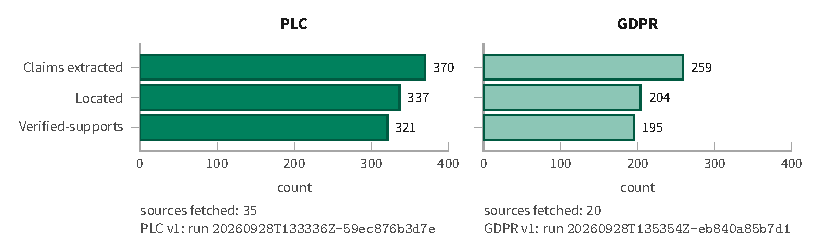
\includegraphics{figures/pdf/fig06_n2.pdf}
  \caption[N2 stage counts]{How much survives each N2 pipeline stage in the two v1 runs (PLC and
  GDPR): sources fetched, claims extracted, located (sidecar \code{n_located}), and verified as
  supported. GDPR loses more than twice the share PLC loses between extraction and location
  (21\% vs.\ 9\%); both lose about 5\% between location and support.}
  \label{fig:n2}
\end{figure}

\subsection{What N2 taught us}

\textbf{Plan the budget as part of the design.} \evint{} A key with a \$5 weekly limit met three
registered experiments whose caps summed to about \$21, and nobody checked headroom against the sum
of caps before running. N2 closed inconclusive partly for a budget reason: the floor failure closed
Continue, and the budget stopped the remaining arms. A pre-run headroom check is now a queued lesson.

\textbf{Silent failures can hide behind a \code{complete: true} flag.} \evobs{} In GDPR v2, 140
verify calls raised and left no trace, yet the sidecar reported \code{complete: true}; the same
provider event most likely cut off E-PLANT's sealed gated run~1. The fix logs every failed attempt
and counts skips per task. \evint{} The fix is partial: \code{complete} and the N3 input flag still
ignore \code{failed_calls_by_task}.

\textbf{Calibrate a \enquote{beats the baseline} gate before registering it.} \evint{} Both
experiments ran their ungated baseline before any gated arm, but nobody computed the reachable range
of the registered gate from it. E-PLANT's floor came from a condition (the plant as the only
context) that E-PLANT did not reproduce. E-ABST's \code{null}-offering schema set an abstention
ceiling the raw model met on its own, 79\% of the time. A future planted-falsehood design needs a
calibration pilot, printed as a \enquote{best reachable outcome}, before any gate is registered.
